\documentclass[11pt]{article}
\usepackage{fancyhdr}
\usepackage{geometry}
\usepackage[shortlabels]{enumitem}
\usepackage{listings}
\usepackage{xcolor}
\usepackage{graphicx}
\usepackage{amsmath}
\usepackage{pdfpages}
\usepackage{float}

\definecolor{codegreen}{rgb}{0,0.6,0}
\definecolor{codegray}{rgb}{0.5,0.5,0.5}
\definecolor{codepurple}{rgb}{0.58,0,0.82}
\definecolor{backcolour}{rgb}{0.95,0.95,0.92}

\lstset{
  backgroundcolor=\color{backcolour},
  commentstyle=\color{codegreen},
  keywordstyle=\color{magenta},
  numberstyle=\tiny\color{codegray},
  stringstyle=\color{codepurple},
  basicstyle=\ttfamily\footnotesize,
  breakatwhitespace=false,
  breaklines=true,
  captionpos=b,
  keepspaces=true,
  showspaces=false,
  showstringspaces=false,
  showtabs=false,
  tabsize=2
}

\fancyhead{}
\fancyfoot{}
\fancyhead[L]{\footnotesize{\textsf{Alex Cutforth | 24375019}}}
\fancyhead[R]{\footnotesize{\textsf{EMTH211, Assignment 2, \today}}}
\fancyfoot[R]{\footnotesize{\textsf{page \thepage}}}
\geometry{
  %showframe,
  includehead,
  includefoot,
  paper      = a4paper,
  top        = 2.0 cm,
  bottom     = 1.0 cm,
  inner      = 2.0 cm,
  outer      = 2.0 cm,
  headheight = 0.5 cm,
  headsep    = 0.5 cm,
  footskip   = 0.5 cm
}

\pagestyle{fancy}

\begin{document}

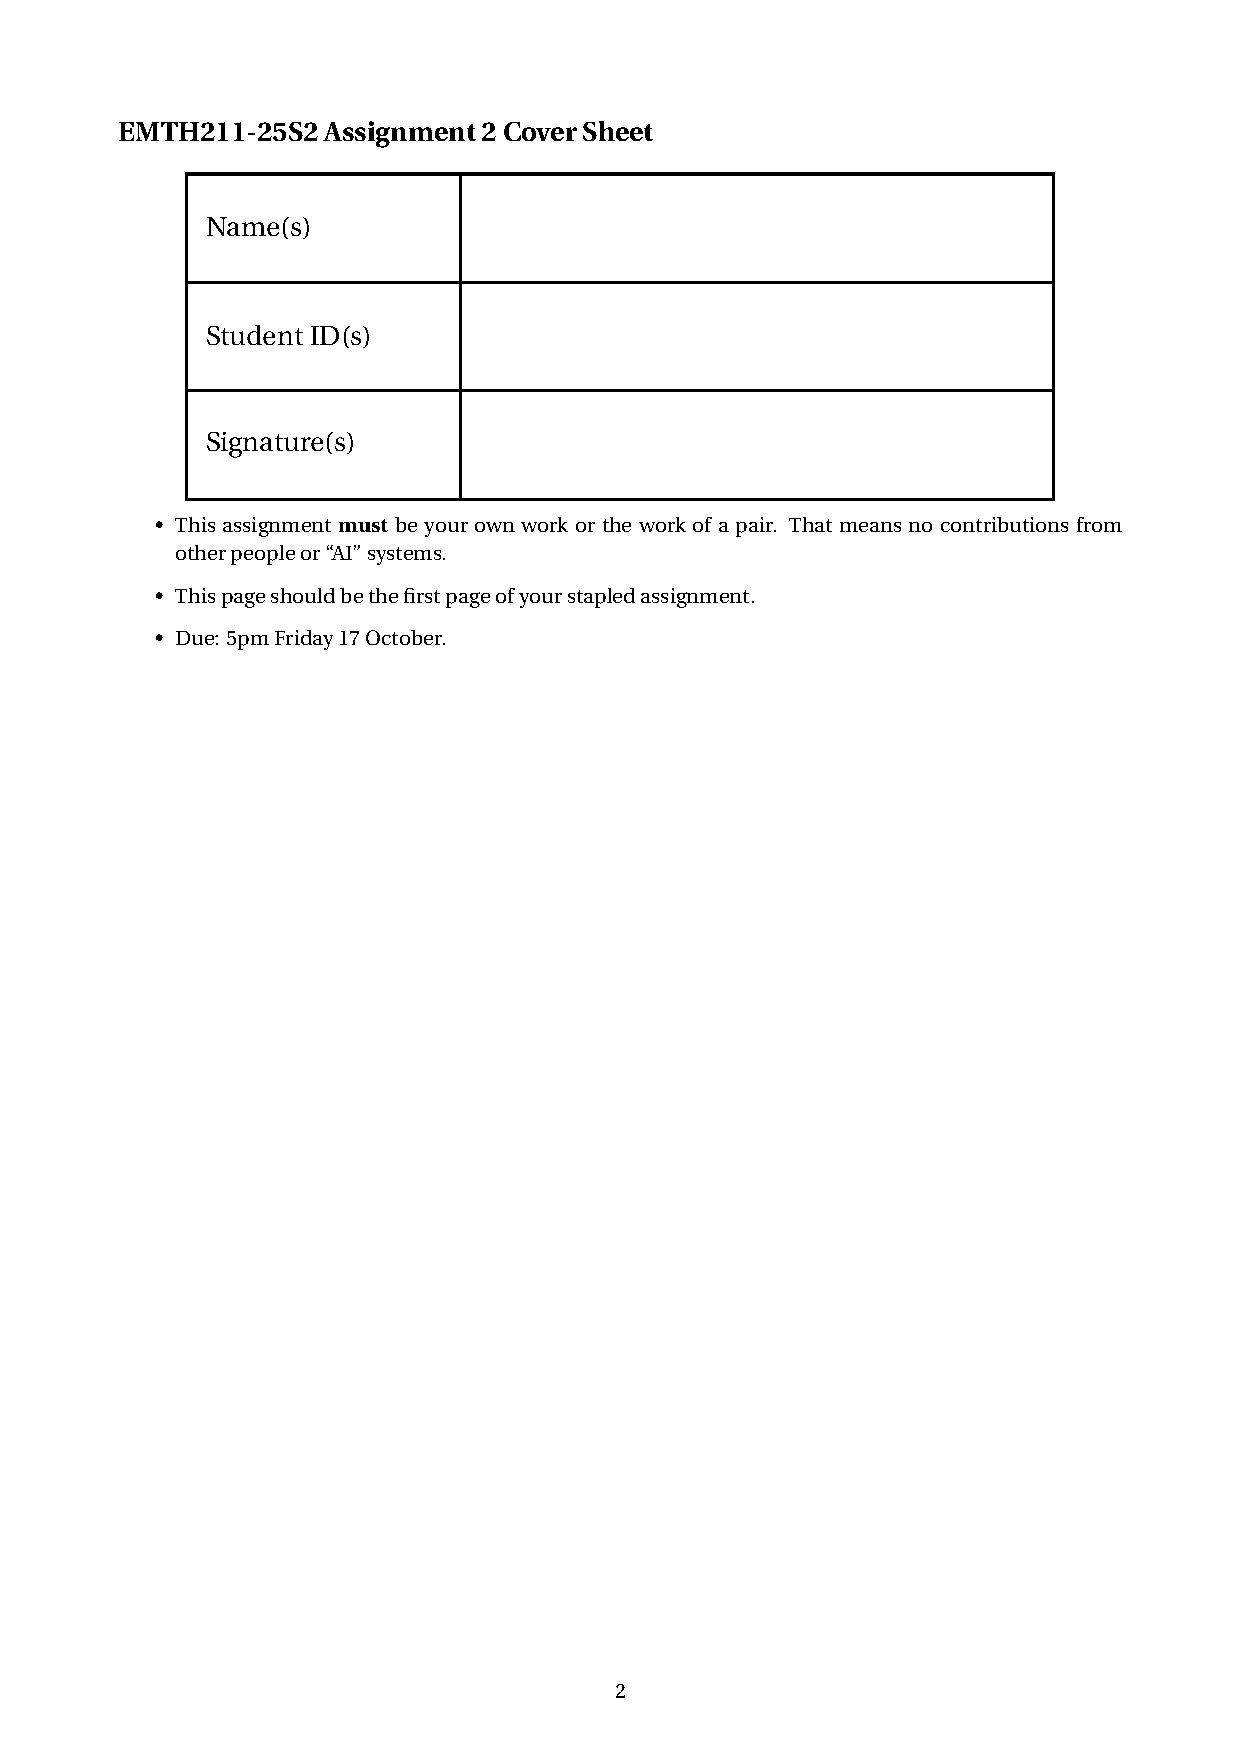
\includepdf[pages=-]{cover-sheet.pdf}

\section*{Question 1}

\begin{enumerate}[a)]
\item ~
  \begin{figure}[h!]
    \centering
    \includegraphics[width=100mm]{1a.graph.png}
    \caption{Plot of maximum floating point operations per second achieved by the fastest supercomputer in each year}
  \end{figure}

\item
  The linear system $A \mathbf{\underline{c}} \approx \mathbf{\underline{y}}$ is structured as:
  $$
  \overbrace{
    \begin{bmatrix}
      1&x_1 \\
      1&x_2 \\
      \vdots&\vdots \\
      1&x_n \\
    \end{bmatrix}
  }^A
  \overbrace{
    \begin{bmatrix}
      c_1 \\
      c_2 \\
    \end{bmatrix}
  }^{\mathbf{\underline{c}}}
  =
  \overbrace{
    \begin{bmatrix}
      \ln{y_1} \\
      \ln{y_2} \\
      \vdots \\
      \ln{y_n}
    \end{bmatrix}
  }^{\mathbf{\underline{y}}}
  $$
  which is represented in code, and solved using QR decomposition in code as:
  \lstinputlisting[language=Python, firstline=4, lastline=8]{part1.py}
  where the vector $\mathbf{\underline{c}}$ is the vector returned from the function.

  This can then be plotted with the code:
  \lstinputlisting[language=Python, firstline=33, lastline=35]{part1.py}
  \begin{figure}[H]
    \centering
    \includegraphics[width=80mm]{1b.graph.png}
    \caption{Maximum Flops per second with line of best fit}
  \end{figure}
\item I will arbitrarily choose 2015 as the split year, this results in the graph:
  \begin{figure}[H]
    \centering
    \includegraphics[width=80mm]{1c.graph.png}
    \caption{Maximum Flops per second with seperate lines of best fit}
  \end{figure}
  This change may be influenced by the fast growth in machine learning and artificial inteligence occuring in the late 2010s vastly increasing the demand for computational power.
  This year may have not been the best point to split the lines, due to the fact that the lines do not connect to each other.
\item The maximum error is computed as such:
  \lstinputlisting[language=Python, firstline=62, lastline=62]{part1.py}
  giving a value of $1.19$.
  \\\\
  Using the line of best fit from the source data, the flops per second in 1969 is extrapolated to be $183977$, however the actual value is known to be $36000000$.
  This means the extrpolation in 1969 had an error of 5.28. This is quite a large error, and speaks to the fact that extrapolation is generally less reliable than interpolation.
  The behavior of the data in the extrapolation region has no effect on the line of best fit, which is why the line of best fit is less reliable at predicting that behavior than that which is inside its range.
\end{enumerate}

\pagebreak
\section*{Question 2}
\begin{enumerate}[a)]
\item The Images I will use for this question are:
\begin{figure}[h!]
  \begin{minipage}{0.48\textwidth}
    \centering
    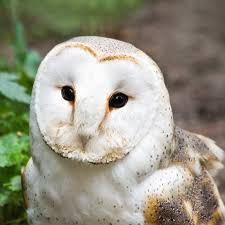
\includegraphics[width=0.7\linewidth]{owl.jpg}
    \caption{Hooty the Owl}\label{fig:owl}
  \end{minipage}
  \begin{minipage}{0.48\textwidth}
    \centering
    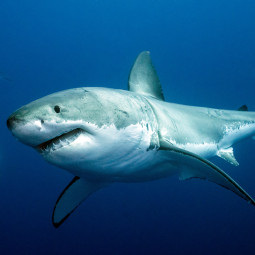
\includegraphics[width=0.7\linewidth]{shark.jpg}
    \caption{Bitey the Shark}\label{fig:shark}
  \end{minipage}
\end{figure}

Part a) doesen't really have an answer to show, but the code for the next parts use the code written for this.
\item
I would say the images need Rank 3 to look vaguely recogniseable.
\begin{figure}[H]
\centering
\includegraphics[width=1\textwidth]{2b.graph.png}
\caption{Approximations up to Rank 5 of Hooty and Bitey}
\end{figure}
The code for finding the rank $r$ approximation of a matrix is:
\lstinputlisting[language=Python, firstline=7, lastline=10]{part2.py}
This is applied to each of the three colour channels (Red, Green, Blue) of each image.
\item
For an $n \times n$ matrix, a total of $k(2n + 1)$ numbers are required for a rank $k$ approximation.
Lossless compression is achieved when k equals the rank of the original matrix.

This means that the maximum rank matrix which can achieve lossless compression is $\frac{n^2}{2n+1}$, which approaches $\frac{1}{2}n$ as n gets large (that is to say, if the rank is higher, a rank r approximation will take more data than the original matrix).

\item While I initially thought the blue channel would be the most important channel for showing the shark, it turns out having a higher rank green channel results in the most crisp image for both Hooty and Bitey.
\begin{figure}[h!]
\centering
\includegraphics[width=1\textwidth]{2d.graph.png}
\caption{Demonstration of Higher rank approximations on specific colour channels}
\end{figure}
\end{enumerate}
\section*{Question 3}

\begin{enumerate}[a)]
\item~
\begin{figure}[h!]
\centering
\includegraphics[width=0.7\textwidth]{3a.graph.png}
\caption{Graph of sin(x) and its 3rd and 4th degree approximations}
\end{figure}

\item Maximum error occurs at $x = 0$. This makes sense since it is the transition between the two peices of the function, so it is not differentiable at that point.
\begin{figure}[h!]
\centering
\includegraphics[width=0.7\textwidth]{3b.graph.png}
\caption{Absolute error of the 4th degree approximation of sin(x)}
\end{figure}

\pagebreak
\item The lowest degree approximation whose maximum error is less than 0.1 is n = 11
\begin{figure}[h!]
\centering
\includegraphics[width=0.7\textwidth]{3c.graph.png}
\caption{11th degree approximation of sin(x)}
\end{figure}

\item
Using Sympy allows us to undertake mathematical operations without having to evaluate the function at specific points.
This also gets rid of any compounding floating point error throughought the multiple integrations which have to occur to create the orthonormal basis and to find approximations from said basis.

A disadvantage of using sympy is it likely took longer to evaluate than using traditional numerical methods.
\end{enumerate}

\pagebreak
\section*{Appendix A: Code}
\subsection*{Question 1}
\lstinputlisting[language=Python]{part1.py}
\subsection*{Question 2}
\lstinputlisting[language=Python]{part2.py}
\subsection*{Question 3}
\lstinputlisting[language=Python]{part3.py}
\end{document}
